% Created 2022-06-02 Thu 11:44
% Intended LaTeX compiler: pdflatex
\documentclass[11pt]{article}
\usepackage[utf8]{inputenc}
\usepackage[T1]{fontenc}
\usepackage{graphicx}
\usepackage{grffile}
\usepackage{longtable}
\usepackage{wrapfig}
\usepackage{rotating}
\usepackage[normalem]{ulem}
\usepackage{amsmath}
\usepackage{textcomp}
\usepackage{amssymb}
\usepackage{capt-of}
\usepackage{hyperref}
\author{Svoronos - Kanavas Iason}
\date{\today}
\title{Construction sites SonVis Algorithm documentation}
\hypersetup{
 pdfauthor={Svoronos - Kanavas Iason},
 pdftitle={Construction sites SonVis Algorithm documentation},
 pdfkeywords={},
 pdfsubject={},
 pdfcreator={Emacs 27.1 (Org mode 9.0.6)},
 pdflang={English}}
\begin{document}

\maketitle
\tableofcontents


\section{Algorithm architecture}
\label{sec:org1f77fbb}
The overall algorithm is structured as:
\begin{enumerate}
\item Interface
\item Sub-processes
\item data processing algorithm
\begin{enumerate}
\item outlier identification,
\item replacement,
\item dataframe creation and manipulation,
\item min-max extraction script
\item datetime re-sample function
\end{enumerate}
\item on-run functions (includes matrix printing functions)
\item IPC inter-process communication (\& connection setup functions)
\item Sonification algorithm
\begin{enumerate}
\item processing functions
\item data receiver -- handler
\item synth and data parameter dictionary
\item event receiver - actions
\item IPC connection configuration
\item synthesisers
\item map to scale frequency mapping patch
\end{enumerate}
\end{enumerate}

\section{Interface}
\label{sec:orgaae3c83}
The interface consists of certain visual elements.
The datetime range slider and text input (for the time) are used for date and time accordingly. Using these the user can specify a desired datetime period in the data to sonify and visualise.

\begin{center}
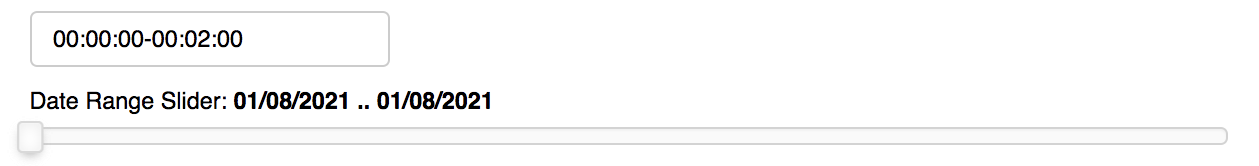
\includegraphics[width=.9\linewidth]{./datetime_selection.png}
\end{center}

The \textbf{start} button is used so that the datetime period is extracted and then sent to be sonified and visualised, while the \textbf{killall} button can interrupt/stop every running procedure in relation to the sonification and visualisation process anytime.

\begin{center}
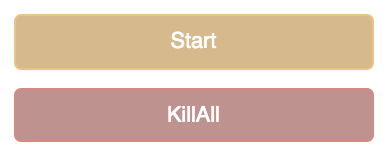
\includegraphics[width=.9\linewidth]{./start_kill_buttons.png}
\end{center}

Below, there is a checkbox where the user can select the period of the values in the data to re-sample.

\begin{center}

\includegraphics[width=.9\linewidth]{./resample_checkbox.png}
\end{center}

The original collection is every 30 seconds.  The re-sample options are, per minute (T), per 30 minutes (30M), per hour (H), per week (W), per month (M).  In the re-sample function (see below), the data values are derived in every period with selecting the max value when doing the frequency conversion to highlight peaks in the data.  For example, if we want to re-sample with 1 minute re-sample frequency (T). We have initially:
\begin{center}
\begin{tabular}{lr}
\hline
timestamp, & data\\
2021-08-01 00:00:00, & 2\\
2021-08-01 00:00:30, & 0\\
2021-08-01 00:01:00, & 4\\
\hline
\end{tabular}
\end{center}

Re-sample result: The extracted value for the first minute will be "4" because is the max value observed for this minute.

Then, there is a another slider that controls the data iteration frequency and it has a range from 1 to 1000 values per second.

\begin{center}
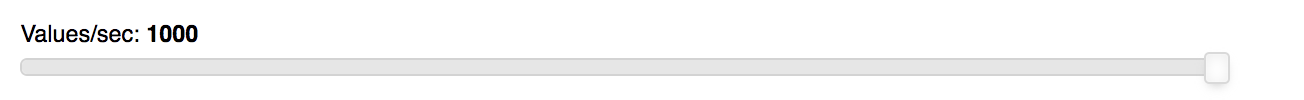
\includegraphics[width=.9\linewidth]{./values_sec.png}
\end{center}

Finally, there are six buttons where the user can use to turn on/off, the desired data parameters to sonify - visualise

\begin{center}
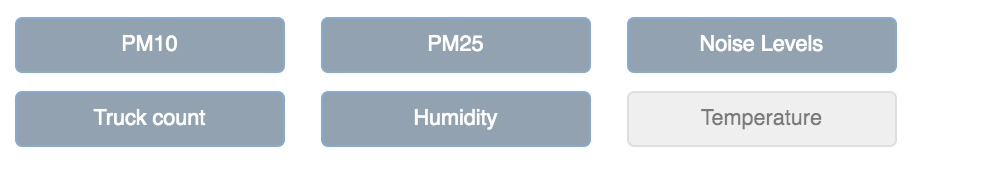
\includegraphics[width=.9\linewidth]{./synth_onoff.png}
\end{center}

\vspace{0.5em}

Overall, the button python bokeh elements, trigger osc messages that are sent from python to supercollider in order to control different synths.
The ones that utilise this functionality is the \textbf{start} \textbf{killall} and the synth on/off buttons (pm10, pm25, temp, humidity, noise levels, truck count).
This will be elaborated in the IPC section

\section{Sub-processes}
\label{sec:org4c5f01e}
On launch, sclang is initialised and runs as a sub-process within the python session.  More specifically, the SuperCollider  patch for sonification is evaluated using the following command in Python.
\begin{verbatim}
# run sonification patch
sclang = subprocess.Popen(
    'sclang particleSonification.scd', shell=True,
    stdout=subprocess.PIPE,
    stderr=subprocess.STDOUT)
\end{verbatim}
Getting back now to the initialisation python script where a function obtains the IP address of the computer using a shell command and then stores it as a global variable.  After that, the OSC client configuration setup uses the variable's value (udp\(_{\text{client}}\) object).  The function is defined the following way as well as the OSC setup.  This process easily configures OSC intercommunication between python and SuperCollider therefore mistakes and hassle by hard-coding IP addresses or manual configurations are avoided.

\begin{verbatim}
# get IP address
def getip():
    global ip
    ip = subprocess.Popen(
        'ipconfig getifaddr en0', shell=True,
        stdout=subprocess.PIPE,
        stderr=subprocess.STDOUT)
    ip, _ = ip.communicate()
    ip = ip.decode('utf-8')
    ip = ip.strip()
    print(ip)

# Python osc
getip() # run getip function
client = udp_client.SimpleUDPClient(ip, 57120)
\end{verbatim}
\textbf{Note:} \emph{this works \textbf{only for macOs}.  Therefore it has to be adjusted for linux or windows.}

\vspace{0.2cm}
\noindent
WIN hint:
\begin{verbatim}
ipconfig | grep IPv4 Address.
\end{verbatim}

\section{data processing}
\label{sec:org048cbec}
In this section the data processing will be described.  The algorithm is developed in Python.  The idea is based on combining and re-constructing the datasets after the processing results that come out from the derived stats (IQR).  SC has also access to the derived dataset (it is written to disk) so that it has access to the min max values for the correct mapping (see \ref{sec:orga3349c2}).  In this way, it is also possible to re-use the algorithm with different data since the mapping is not hard-coded.

Outlier identification and replacement was deemed necessary since it was observed by using box-plot stats the PM (both 25 and 10) showed extreme values (far from accurate measurements (140\textasciitilde{} PM10) ) that we would like to exclude.

\begin{center}
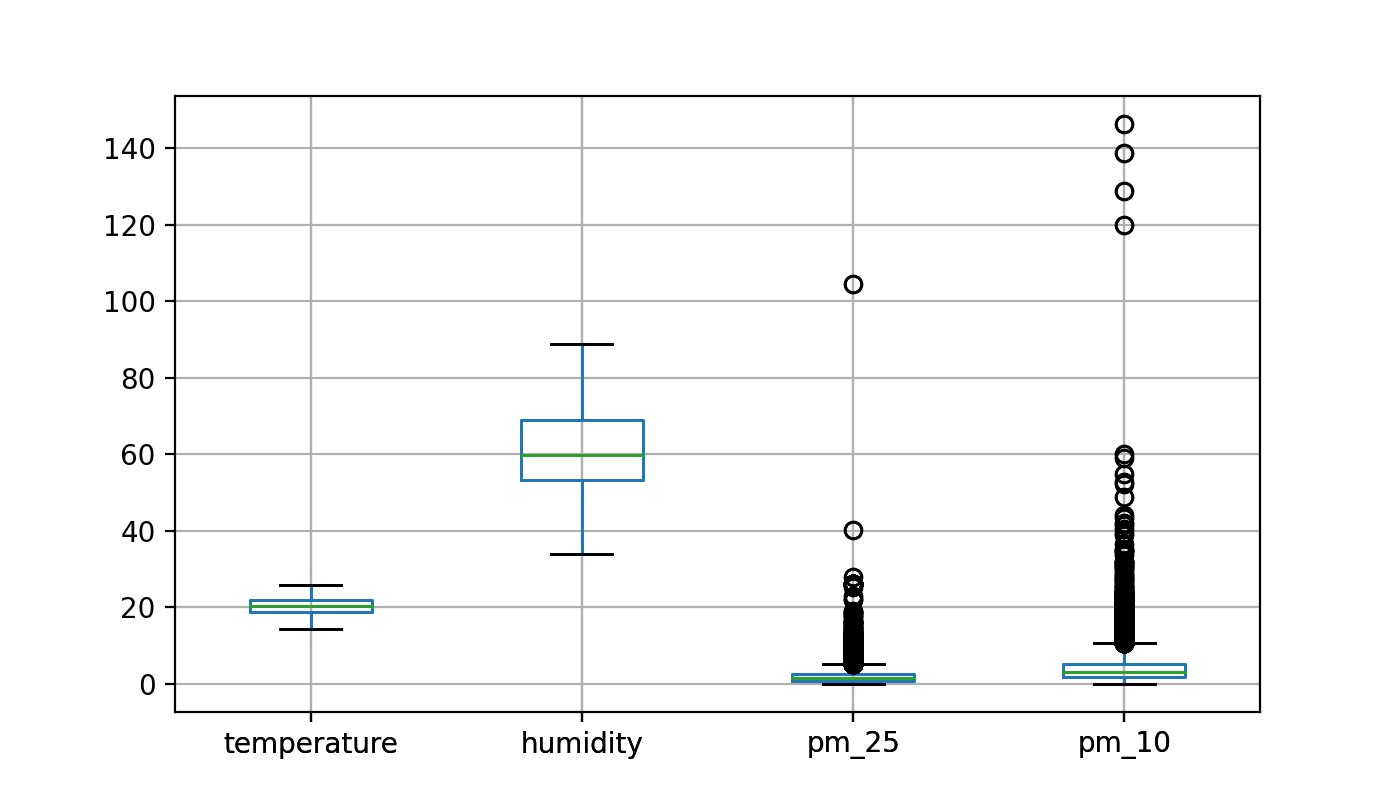
\includegraphics[width=.9\linewidth]{./boxplot.png}
\end{center}

\subsection{outlier identification}
\label{sec:orga32c40a}
\subsection{replacement}
\label{sec:org7f1f43f}
\subsection{dataframe creation and manipulation}
\label{sec:orgad4ee46}
\subsection{min-max extraction script}
\label{sec:orga3349c2}
\subsection{datetime re-sample function}
\label{sec:org1adad15}
\section{on-run functions}
\label{sec:orgb5526f4}
\section{IPC inter-process communication (includes connection setup functions)}
\label{sec:orgfe3fee3}
\section{Sonification algorithm}
\label{sec:org80b7ab9}
\subsection{processing functions}
\label{sec:org6c644b6}
\subsection{data receiver -- handler}
\label{sec:org0d991e2}
\subsection{synth and data parameter dictionary}
\label{sec:org5c8a463}
\subsection{event receiver - actions}
\label{sec:org5207646}
\subsection{IPC connection configuration}
\label{sec:org0657bc8}
\subsection{synthesisers}
\label{sec:org0f9dc78}
\subsection{map to scale frequency mapping patch}
\label{sec:orgb11469d}
\end{document}
